\chapter{Agentic AI} 

Agentic AI describes a comprehensive AI system that can make decisions and perform actions for either general or specific tasks, with minimal human intervention. It is a fundamental building block of autonomous systems.

The concept of agentic AI is not new. However, in recent years it has drawn increasing attention due to the rapid advancements in LLM. LLMs provide a general-purpose language interface that makes agentic AI significantly more scalable and cost-effective. As a result, agentic AI is included as a key topic in this part of the notebook.

\section{Introduction to Agentic AI}

The term ``agent'' refers to an entity that acts on behalf of a human. By this definition, agentic AI refers to AI-based systems that can solve complex problems with limited human oversight. This idea predates LLMs. However, with the rise of LLMs, the term ``agentic AI'' has been re-contextualized and is experiencing renewed popularity.

We explore agentic AI from two perspectives:

\begin{itemize}
  \item Conventional intelligent agents. Classical agents developed in traditional AI literature before the rise of LLMs.
  \item LLM-driven agentic AI. Modern, language-enabled agents powered by large language models.
\end{itemize}

More details are given in the rest of the section.

\subsection{Conventional Intelligent Agent}

TBA

\subsection{Agentic AI in the Context of LLM}

Agentic AI in the context of LLMs refers to an autonomous system in which LLMs not only perform tasks, but also participate in decision-making and workflow orchestration. In such systems, LLMs serve both as computational units that solve sub-tasks and as the high-level orchestrator that determines how the problem should be approached.

An LLM in an agentic AI system may take on one or more of the following roles:
\begin{itemize}
	\item Decompose the original problem into smaller sub-problems.
	\item Assign these sub-problems to LLM instances, either sequentially or in parallel.
	\item Evaluate the outputs of LLMs and either accept the results or reject them with feedback and revision instructions.
	\item Integrate the outputs from sub-problems into a final, coherent solution to the original problem.
\end{itemize}

In contrast, conventional LLM-integrated applications rely on humans or pre-written deterministic code to perform all of the above tasks. From this perspective, agentic AI further reduces human intervention and increases the level of automation.

A comparison is illustrated in Fig.~\ref{fig:agenticwf1}. In the conventional architecture shown in (a), the workflow is either hard-coded or defined externally, and the LLM merely serves as a problem solver. In the agentic AI architecture shown in (b), the LLM autonomously orchestrates the task, determines the workflow, and governs the solution process.

\begin{figure}[!htb]
	\centering
	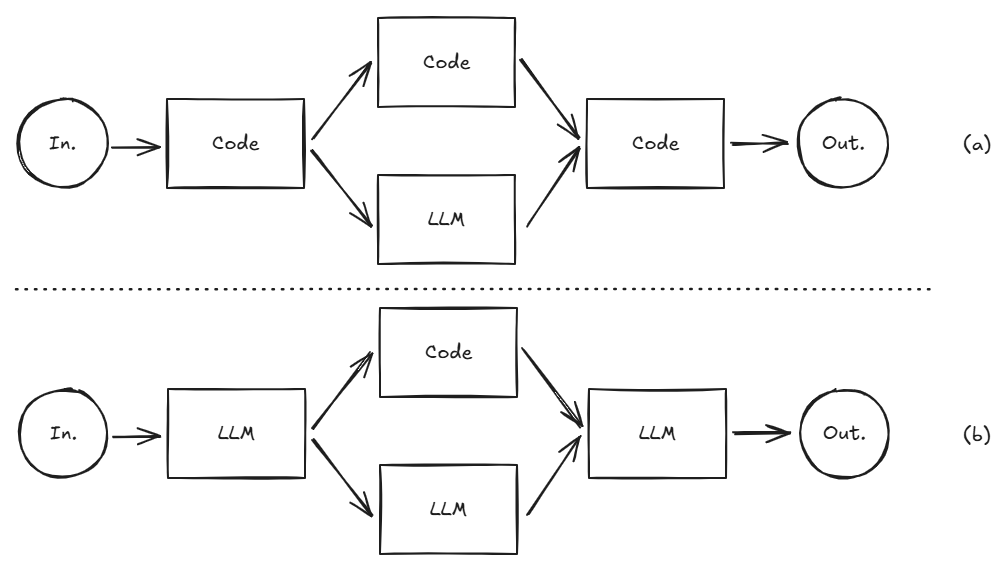
\includegraphics[width=\textwidth]{./chapters/part-7/figures/agenticaiworkflow.png}
	\caption{Conventional architecture (a) versus agentic AI architecture (b).}
	\label{fig:agenticwf1}
\end{figure}

Figure~\ref{fig:agenticwf1} is not the only architectural pattern for agentic AI. Another commonly used architecture is shown in Fig.~\ref{fig:agenticwf2}. In this design, one LLM generates an output while another LLM evaluates its quality, decides whether to accept or reject it, and provides revision instructions if necessary. The two LLMs collaborate in an iterative loop, refining the solution step by step. This self-evaluative architecture has been shown to significantly reduce the likelihood of low-quality or hallucinated outputs.

\begin{figure}[!htb]
	\centering
	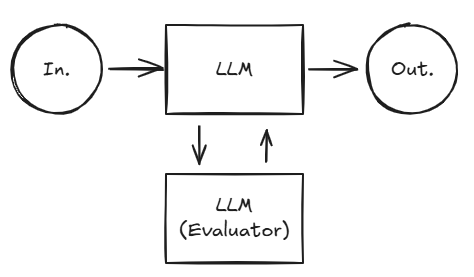
\includegraphics[width=0.5\textwidth]{./chapters/part-7/figures/agenticaiworkflow2.png}
	\caption{Self-evaluative agentic AI architecture.}
	\label{fig:agenticwf2}
\end{figure}

Another key feature of LLM-based agentic AI is that it does not rely solely on the internal knowledge encoded in the model. Instead, it can be configured to interact with external tools such as databases, web browsers, calculators, etc., to enhance its problem-solving capabilities. This tool-augmented reasoning is essential for tasks that require up-to-date information, precise computation, or direct interaction with external environments. It also helps with reducing hallucination. A representative architecture is given in Fig.~\ref{fig:agenticwf3}, where the LLM autonomously decides when to invoke an external tool and generates the appropriate commands using pre-defined protocols known as the \mync{Message Communication Protocol}[MCP]. More details are given in later sections.

\begin{figure}[!htb]
	\centering
	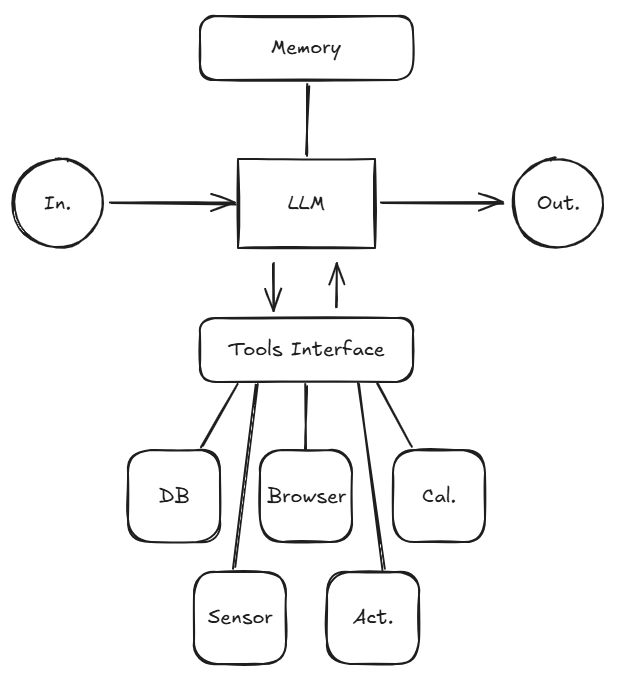
\includegraphics[width=0.8\textwidth]{./chapters/part-7/figures/agenticaiworkflow3.png}
	\caption{LLM with memory and tool interfaces to databases, web browsers, calculators, sensors and actuators, and other components that can interact with the environment.}
	\label{fig:agenticwf3}
\end{figure}

Recall RAG which focuses on database-integrated LLMs to expand knowledge boundaries and suppress hallucinations. A fully developed agentic AI can be taken as an extension of RAG.

In addition, the LLM is equipped with a memory module, which stores historical inputs and outputs to maintain context and support long-term reasoning. This is also shown in Fig.~\ref{fig:agenticwf3}.

\section{Agentic AI Framework}

Agentic AI can be understood as a form of LLM orchestration. The user specifies the overall task and provides a list of available tools, while the agentic AI system determines how to structure the workflow, which tools to invoke, how to prompt the LLMs, and how to evaluate their outputs.

An \mync{agentic AI framework} refers to the infrastructure that supports the creation, configuration, and execution of such systems. It provides the necessary abstractions and utilities that allow users to define and deploy agentic AI pipelines more easily. While it is always possible to manually coordinate LLMs, prompts, and tool calls, using a mature agentic AI framework significantly simplifies the process of building scalable, multi-agent, or tool-augmented systems.

In this sense, an agentic AI framework plays a role analogous to that of Kubernetes in the context of containerized applications: it abstracts away low-level orchestration logic and enables the declarative specification and runtime management of complex, distributed components.

Common examples of agentic AI frameworks include the OpenAI Agents SDK, CrewAI, LangGraph, AutoGen, and many more. Details are introduced in later sections.

\subsection{Asynchronous Python}

Before introducing different agentic AI frameworks, it is worth reviewing asynchronous Python programming, as it is widely used across many agentic AI platforms.

Asynchronous programming (often abbreviated as async programming) is a well-established concept that predates agentic AI. In a nutshell, it creates a ``multi-thread-like'' framework where functions do not necessarily run in the order they are defined, but instead follow a ``first-ready, first-served'' execution model. In the context of async Python programming, an event loop switches between tasks whenever one is waiting (typically due to I/O). It is multi-thread-like in behavior, but there is no true CPU-level parallelism and no true multithreading. By itself, \verb|asyncio| runs on a single thread and a single CPU core; true CPU-bound parallelism requires multiprocessing or native threads.

Even before the emergence of agentic AI frameworks, async programming had already proven valuable in many applications, such as web servers handling HTTP requests or user interfaces monitoring human actions on dashboards. By using async programming, an application does not need to freeze while a task is waiting for inputs—usually from a user or over the internet—and can continue executing other tasks in the meantime.

The \verb|asyncio| library is the standard Python library for writing concurrent code using the \verb|async|/\verb|await| syntax, and many other async libraries are built on top of it. A detailed introduction to \verb|asyncio| can be found at \cite{python2025asyncio}. A brief review of the basic syntax is given below.

The basic syntax to define and run a Python \mync{coroutine function} is as follows:
\begin{lstlisting}
import asyncio

async def <coroutine_function_name>(input) -> output:
    <do something; can contain nested coroutines>
    [return <something>]
    
[result = ]asyncio.run(<coroutine_function_name>(input))
\end{lstlisting}
Here, \texttt{async def} defines a coroutine function, and calling it returns a coroutine object. The function \texttt{asyncio.run()} runs the given coroutine object as the main entry point of the program. It creates and manages the event loop, runs the coroutine until it is complete, and then closes the loop. This approach is particularly useful when multiple coroutines are executed inside the main coroutine.

Calling a coroutine function directly, as in the example below, does not run it immediately; instead, it returns a coroutine object:
\begin{lstlisting}
[<coroutine_object> = ]<coroutine_function_name>(input) # does not execute
\end{lstlisting}
In this case, the result is a coroutine object rather than the calculation’s output. This coroutine object can then be scheduled and executed as follows:
\begin{lstlisting}
[result = ]asyncio.run(<coroutine_object>)
\end{lstlisting}
When executing a coroutine object like this, there is no need to pass its input arguments again. A coroutine object can be awaited only once.

Another way to execute a coroutine is with the \verb|await| expression:
\begin{lstlisting}
[result = ]await <coroutine_function_name>(input)
\end{lstlisting}
However, this syntax can only be used inside another coroutine. It cannot be used at the top level, because \verb|await| requires an already running event loop. What it does is suspend the current coroutine until the awaited coroutine completes, allowing the event loop to run other tasks in the meantime.

The \texttt{asyncio.gather()} function is another way to schedule multiple coroutines concurrently on the same event loop. For example:
\begin{lstlisting}
x = await cx()
y = await cy()

x, y = await asyncio.gather(
    cx(), 
    cy()
)
\end{lstlisting}
In the first approach, \verb|cx| and \verb|cy| are executed sequentially. If \verb|cx| is delayed due to I/O, \verb|cy| must wait until \verb|cx| finishes. During this time, the event loop may run other ready-to-execute tasks. In the second approach, \verb|cx| and \verb|cy| are scheduled concurrently. While \verb|cx| is waiting for inputs, \verb|cy| can still execute. If both are waiting, \verb|asyncio.gather| pauses, and the event loop switches to other tasks.

The same principle applies to the entire event loop. If the whole event loop is paused (its ready queue is empty), it uses the OS-level selector to wait for I/O readiness, and the operating system schedules other work until new events are ready.

\subsection{OpenAI Agents SDK} \label{sec:openaisgentssdk}

The OpenAI Agents SDK simplifies the deployment of an agentic AI system without sacrificing flexibility. In fact, it enables more versatile agentic AI pipelines, such as chaining multiple AI agents using handoffs and nesting AI agents within tools-capabilities that would be almost impossible to implement manually due to the complexity of such systems.

The OpenAI Agents SDK offers at least the following features:
\begin{itemize}
	\item Simplified deployment of a single AI agent or tool.
	
	For example, when defining a tool manually, the user must create a detailed “user manual” in JSON object format and pass it to the LLM. This JSON must include the tool’s name, description, and input arguments with their types—carefully specified to ensure correct behavior. With the OpenAI Agents SDK, the user can simply add a decorator to a Python function to turn it into a tool, without needing to write a separate descriptive JSON object.
	
	\item Easy conversion of AI agents into tools.
	
	A single-line command can convert an AI agent into a tool, enabling nested structures. This significantly increases the capabilities of higher-level AI agents that use these tools.
	
	\item Chaining AI agents using handoffs. 
	
	Information processed by an upstream AI agent can be passed to a downstream agent easily via \mync{handoffs}, a mechanism for explicitly transferring control and data between agents during execution. The upstream agent decides when and where to pass the data. This allows true cooperation between AI agents and enables highly flexible agentic AI pipelines.
\end{itemize}

Figure \ref{fig:openai_agents_sdk_pipeline} illustrates the key features of the OpenAI Agents SDK compared with a manual implementation. As shown, in the SDK-based pipeline, an AI agent can be converted into a tool and respond to tool calls (red arrows). Multiple AI agents can also be chained to form an upstream–downstream pipeline via handoffs (blue arrows). When an AI agent has multiple possible downstream agents, it can decide at runtime which one to hand over data and control to.

\begin{figure}[!htb]
	\centering
	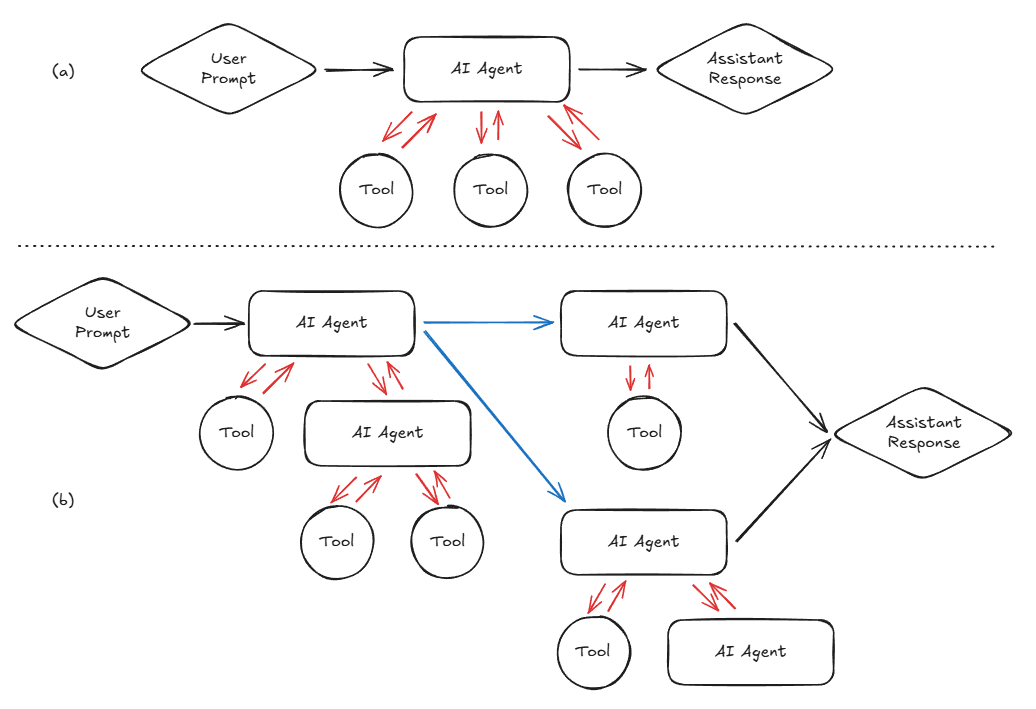
\includegraphics[width=\textwidth]{./chapters/part-7/figures/openai_agents_sdk_pipeline.png}
	\caption{Manually implemented (a) versus OpenAI Agents SDK–based (b) agentic AI pipelines. Red arrows represent tool calls, and blue arrows represent handoffs.}
	\label{fig:openai_agents_sdk_pipeline}
\end{figure}

The basic syntax is introduced below. All code examples are assumed to be executed in an environment with a running event loop. One can assume a wrapper as follows. Note that \verb|OPENAI_API_KEY| is also assumed to be loaded as an environment variable.

\vspace{0.1in}
\noindent \textbf{Agent}
\vspace{0.1in}

\begin{lstlisting}
import asyncio
from dotenv import load_dotenv

async def main():
    load_dotenv(override=True)
    
    <the code to be introduced>

if __name__ == "__main__":
    asyncio.run(main())
\end{lstlisting}

The following example demonstrates how to create an agent with a system prompt and a user prompt.

\begin{lstlisting}
from agents import Agent, Runner, trace, function_tool

system_prompt = "<system prompt>"

agent_instance = Agent(
    name="<agent name>",
    instructions=system_prompt,
    model="<model>"
)
response = Runner.run(<agent name>, "<user prompt>")
output = response.final_output
\end{lstlisting}

The following code is useful when running multiple agents concurrently:
\begin{lstlisting}
with trace("<trace name>"):
    results = await asyncio.gather(
        Runner.run(<agent name 1>, "user prompt 1"),
        Runner.run(<agent name 2>, "user prompt 2"),
        Runner.run(<agent name 3>, "user prompt 3"),
    )
outputs = [result.final_output for result in results]
\end{lstlisting}

The call to \texttt{await asyncio.gather()} works here because an event loop wrapper is already assumed. The function \texttt{asyncio.gather()} schedules all provided coroutines to run concurrently. Notice that the results will be returned in the same order as the input arguments regardless of which coroutine completes first. 

The \verb|trace()| context manager allows the user to monitor all LLM-related calls made to OpenAI, and these traces can be viewed on the OpenAI dashboard.

\vspace{0.1in}
\noindent \textbf{Tool}
\vspace{0.1in}

There are at least two ways to define a tool for an agent, as shown below.

\begin{lstlisting}
@function_tool
def <tool 1>(<input 1>: <input type 1>, <input 2>: <input type 2>, ...):
    """<description>"""
    <do something>
    return {"status": "success", <other returns>}

<tool 2> = <low tier agent name>.as_tool(
    tool_name="<tool name>",
    tool_description="tool description"
)

tools = [<tool 1>, <tool 2>]

agent = Agent(
    name="<high tier agent name>",
    instructions="<system prompt>",
    tools=tools,
    model="<model>"
)
\end{lstlisting}

The first method uses the \verb|@function_tool| decorator and is intended for precise tools such as calculators or database query functions. It requires an explicit list of typed input arguments and returns well-defined, structured results.

The second method uses another low-tier agent as a smart tool via \verb|as_tool|. The input to this tool is simply a string, which is treated as the user prompt for the low-tier agent. This creates a nested structure. The low-tier agent can call its own precise or smart tools, enabling more flexible and modular agentic AI pipelines.

\vspace{0.1in}
\noindent \textbf{Handoff}
\vspace{0.1in}

Handoffs are used to transfer data between agents. In this context, a handoff allows data generated by an upstream agent to be passed to a downstream agent. Downstream agents are registered as available handoffs, and the upstream agent can decide when and where to pass the data.

For a downstream agent, use \verb|handoff_description| as a ``self introduction'' which will be presented to the upstream agent. An example is shown below:
\begin{lstlisting}
downstream_agent = Agent(
    name="<name>",
    instructions="<instructions>",
    tools=[<tool 1>, <tool 2>, ...],
    model="<model>",
    handoff_description="<handoff description>"
)
\end{lstlisting}

List all available downstream agents and provide this list to an upstream agent. The upstream agent can then decide at runtime when to pass data and which downstream agent to use.
\begin{lstlisting}
handoffs = [<downstream_agent 1>, <downstream_agent 2>, ...]
upstream_agent = Agent(
    name="<name>",
    instructions="<instructions>",
    tools=[<tool 1>, <tool 2>, ...],
    model="<model>",
    handoffs=handoffs
)
\end{lstlisting}

It is recommended to include clear instructions in the \verb|instructions| (system prompt) of the upstream agent on how and when to use the downstream agents.

Run the upstream agent, and it will automatically trigger the downstream agents if, based on its instructions and reasoning, it decides to do so. The return value will be the final result of the entire pipeline. Note that handoffs do not force an upstream agent to pass data. It is possible for the upstream agent to return its response directly to the user, completely bypassing the downstream pipeline. In this sense, an upstream agent determines the execution path of the pipeline from itself onward.

\vspace{0.1in}
\noindent \textbf{Guardrail}
\vspace{0.1in}

It is recommended to double-check both the initial user input and the final output of an agentic AI system to ensure that the input meets the required criteria or contains the necessary information, and that the output does not include harmful content.

There are several ways to achieve this. For example, OpenAI provides a moderation API that checks whether a piece of multimodal content contains material related to sexual content, hate, self-harm, and other restricted categories. More about this API will be introduced later in this section, and it will be tested in the project examples.

Within the OpenAI Agents SDK, guardrails can be implemented by defining dedicated AI agents to check the input and output of the agentic AI system according to customized requirements. Such guardrail agents return a boolean flag indicating whether the guardrail was triggered, along with details about what content caused the trigger. If a guardrail is triggered, it will raise an exception.

The following syntax demonstrates the minimum implementation of a guardrail. It involves the following steps.
\begin{enumerate}
	\item Define a class to hold the return value of the guardrail agent. 
	\item Define the guardrail agent itself.  
	\item Define a coroutine function, decorated with \verb|@input_guardrail| or \verb|@output_guardrail|, that triggers the guardrail agent.
\end{enumerate}

\begin{lstlisting}
from pydantic import BaseModel
from openai_agents import Agent, Runner, input_guardrail, output_guardrail, GuardrailFunctionOutput


class <guardrail return class>(BaseModel):
	<is_triggered>: bool
	<reason or content>: str

guardrail_agent = Agent(
	name="<guardrail check agent name>",
	instructions="<instructions, often the things to check>",
	output_type=<guardrail return class>,
)

@output_guardrail
async def <guardrail coroutine name>(ctx: RunContextWrapper, agent: Agent, output: MessageOutput) -> GuardrailFunctionOutput:
	result = await Runner.run(guardrail_agent, output.response, context=ctx.context)
	return GuardrailFunctionOutput(output_info=result.final_output,tripwire_triggered=result.final_output.<is_triggered>)
\end{lstlisting}

When defining an agent in the pipeline, include the above coroutine function as a guardrail:

\begin{lstlisting}
agent = Agent( 
	name="Customer support agent",
	instructions="<instructions>",
	output_guardrails=[<guardrail coroutine name>],
)
\end{lstlisting}

The above example defines an output guardrail. An input guardrail can be defined in a similar way.

Notice that in OpenAI Agents SDK, \verb|input_guardrails| only run when attached to the \emph{first} agent in a chain (on the initial user input), and \verb|output_guardrails| only run when attached to the \emph{last} agent (on the final agent output). Guardrails attached to intermediate agents do not trigger.

Recall that OpenAI provides moderate API to check whether a content contains harmful information. It can be used as the output guardrail as follows.
\begin{lstlisting}
@output_guardrail
async def moderation_guardrail(ctx, agent: Agent, message):
	response = client.moderations.create(
		model="omni-moderation-latest",
		input=message.response
	)
	flagged = response.results[0].flagged
	return GuardrailFunctionOutput(output_info=response.results[0],tripwire_triggered=flagged)
\end{lstlisting}

An example using OpenAI Agents ADK is given in Section \ref{sec:agentaiexp-agentsdk}.

\subsection{CrewAI}

CrewAI is not just a framework but also a company and an ecosystem. Depending on the context, CrewAI can refer to the following:
\begin{itemize}
	\item A company that develops and provides agentic AI solutions.
	\item A platform offered by CrewAI to deploy agentic AI systems on the cloud.
	\item An application with a graphical interface that allows users to design and deploy agentic AI pipelines with minimal coding.
	\item An open-source agentic AI framework.
\end{itemize}
In this notebook, we will focus on the CrewAI framework.

Recall the OpenAI Agents SDK introduced in Section~\ref{sec:openaisgentssdk} and Fig.~\ref{fig:openai_agents_sdk_pipeline}, where the user defines agents, tools, and handoffs, and links them together, while the agents decide which tools and handoffs to use. The CrewAI framework follows a very different philosophy. A ``Crew'' in this context is a team (e.g., engineering, data science, or marketing), where each AI agent acts as an employee. A job is assigned to the team, with specified context, inputs, and outputs. The user plays the role of a ``hiring manager'', defining the roles and characteristics of each AI agent, the context and goals of each task, and assembling the team from scratch. Once all agents and tasks are defined, the team completes the job. This is demonstrated by Fig. \ref{fig:crewai_pipeline}.

\begin{figure}[!htb]
	\centering
	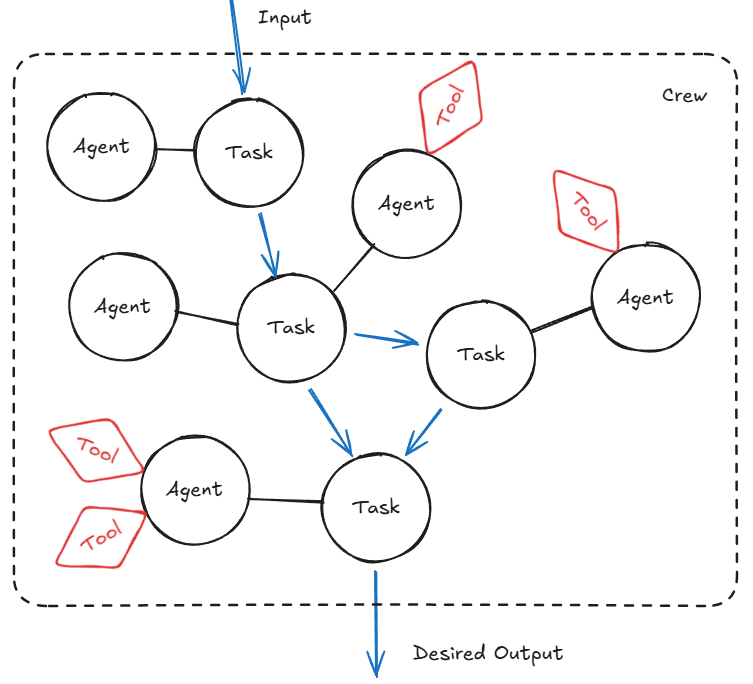
\includegraphics[width=0.8\textwidth]{./chapters/part-7/figures/crewai.png}
	\caption{CrewAI framework pipeline, where the user defines agents, tasks and their associations and the crew get things done automatically.}
	\label{fig:crewai_pipeline}
\end{figure}

In this sense, while the OpenAI Agents SDK requires the user to micro-manage pipeline details, CrewAI emphasizes macro-management by defining context, inputs and outputs, and assigning agents to tasks. The OpenAI Agents SDK is more flexible, but when a job aligns well with CrewAI's philosophy, implementing it in CrewAI is often much easier.

\vspace{0.1in}
\noindent \textbf{CrewAI Installation as a UV Tool}
\vspace{0.1in}

CrewAI provides both Python libraries and CLI tools. It is recommended to install both when working with CrewAI. The CLI tool simplifies project setup by generating a directory tree with template Python scripts that can be adapted for specific applications. Manually creating such a structure from scratch would be tedious.

To install or update CrewAI as a tool with \verb|uv|, use:
\begin{lstlisting}
uv tool install crewai
uv tool install crewai --upgrade
\end{lstlisting}

Once CrewAI is installed, a new project can be created with:
\begin{lstlisting}
crewai create crew <project_name>
\end{lstlisting}

This command generates a project root folder containing a hello-world-style template. During creation, the user is prompted to select a default LLM service provider and model, and to provide an API key. These choices are used in generating the template but can be modified later.

An example of the template directory structure is shown below \cite{crewai2025install}:
\begin{lstlisting}
my_project/
|-- .gitignore
|-- knowledge/
|-- pyproject.toml
|-- README.md
|-- tests/
|-- .env
\-- src/
  \-- my_project/
    |-- __init__.py
      |-- main.py
      |-- crew.py
      |-- tools/
      |  |-- custom_tool.py
      |  \-- __init__.py
      \-- config/
        |-- agents.yaml
        \-- tasks.yaml
\end{lstlisting}

\vspace{0.1in}
\noindent \textbf{Agents and Tasks Definition}
\vspace{0.1in}

In the project template, \verb|agents.yaml| and \verb|tasks.yaml| are configuration files that specify the properties of agents and tasks. An \emph{agent} refers to an LLM with defined capabilities and tools, while a \emph{task} represents a workflow step with input, desired output, and context. These configuration files may include prompts, parameters, and other metadata that shape the agent’s behavior and the execution of tasks.

For example, in a document-refinement workflow, the agent might be a ``publication editor,'' and the task could be ``correct-grammar-error.'' The input would be text containing grammatical mistakes, and the output would be error-free text that preserves the original meaning with minimal changes.

Below is an example of \verb|agents.yaml| created during project initialization.
\begin{lstlisting}
researcher:
  role: >
    {topic} Senior Data Researcher
  goal: >
    Uncover cutting-edge developments in {topic}
  backstory: >
    You're a seasoned researcher with a knack for uncovering the latest developments in {topic}. Known for your ability to find the most relevant information and present it in a clear and concise manner.

reporting_analyst:
  role: >
    {topic} Reporting Analyst
  goal: >
    Create detailed reports based on {topic} data analysis and research findings
  backstory: >
    You're a meticulous analyst with a keen eye for detail. You're known for your ability to turn complex data into clear and concise reports, making it easy for others to understand and act on the information you provide.
\end{lstlisting}

Here, two agents, ``researcher'' and ``reporting analyst,'' are defined. Each agent has three key components: \verb|role|, \verb|goal|, and \verb|backstory|. Together, these specify the agent’s intended capabilities and behavior.
The symbol \verb|>| in YAML indicates a folded block scalar, meaning that multi-line text is treated as a single string with line breaks converted to spaces. The placeholder \verb|{topic}| in the example will be filled dynamically by the higher-level script.

In addition to the compulsory \verb|role|, \verb|goal|, and \verb|backstory| fields, other optional fields may be included. A commonly used one is \verb|llm|, which lets the user specify an LLM model other than the default. For example:
\begin{lstlisting}
<agent_name>:
  role: <something>
  goal: <something>
  backstory: <something>
  llm: openai/gpt-5-mini
\end{lstlisting}
A full list of allowed fields can be found at \cite{crewaiAgentsConcepts}, including tools, agents as tools, maximum iteration number, maximum LLM request rate, etc.

Below is an example of \verb|tasks.yaml| created during project initialization.
\begin{lstlisting}
research_task:
  description: >
    Conduct a thorough research about {topic}. Make sure you find any interesting and relevant information given the current year is {current_year}.
  expected_output: >
    A list with 10 bullet points of the most relevant information about {topic}
  agent: researcher

reporting_task:
  description: >
    Review the context you got and expand each topic into a full section for a report. Make sure the report is detailed and contains any and all relevant information.
  expected_output: >
    A fully fledged report with the main topics, each with a full section of information. Formatted as markdown without '```'
  agent: reporting_analyst
\end{lstlisting}

\subsection{LangGraph}

\subsection{AutoGen}

\section{Examples}

Demonstrative projects are given as examples for a variety of agentic AI applications. 

\subsection{Manual: Semantic Search RAG}

This section demonstrates a manually implemented retrieval‑augmented agent. Documents (papers, reports, web pages, etc.) are stored locally. The agent answers user questions about these documents. Because the total corpus can be large, it is impractical to send all text to the LLM on every turn. Instead, the system performs semantic search to select only the most relevant chunks.

On first run, the program checks whether embeddings already exist locally. If not found, it chunks the documents into pieces with a specified token budget and uses OpenAI’s vector embeddings API to compute vector representations. These vectors are cached locally. On subsequent runs, the cached embeddings are loaded.

On each user request, the query is embedded and used to retrieve the most relevant chunks. These chunks are appended to the prompt and sent to the LLM. The LLM is given an explicit ``retrieval'' tool. If it determines that more context is needed, it may trigger another semantic search with refined keywords or increase the number of returned chunks, or both. This can be performed as many times as the LLM requires.

Dialogues are stored locally so conversations persist across sessions. Only the user’s messages and the assistant’s replies are saved. Retrieved chunks are treated as ephemeral context and are not stored in the conversation log.

The implementation is framework‑free (no agent framework) and can be found at \cite{sun2025document}. Key components are outlined below.

\vspace{0.1in}
\noindent \textbf{Chunk Documents}
\vspace{0.1in}

The following codes are relevant to the chunk of documents.

\begin{lstlisting}
def set_tokenizer(self):
    self.tokenizer = tiktoken.encoding_for_model(self.LLM_EMBEDDING_MODEL)

def tokenize(self, text):
    return self.tokenizer.encode(text)

def count_tokens(self, text):
    return len(self.tokenize(text))

def chunk_text(self, text):
    words = text.split()
    chunks = []
    chunk = []
    tokens_so_far = 0
    for word in words:
        token_count = self.count_tokens(word)
        if tokens_so_far + token_count > self.MAX_TOKENS:
            chunks.append(" ".join(chunk))
            if self.OVERLAP > 0:
                chunk = chunk[-self.OVERLAP:]
                tokens_so_far = self.count_tokens(" ".join(chunk))
            else:
                chunk = []
                tokens_so_far = 0
        chunk.append(word)
        tokens_so_far += token_count

    if chunk:
        chunks.append(" ".join(chunk))

    return chunks

def chunk_documents(self):
    chunks = []
    for filename in os.listdir(self.DOC_DIR_PATH):
        if filename.endswith('.pdf'):
            doc_path = os.path.join(self.DOC_DIR_PATH, filename)
            doc = fitz.open(doc_path)
            text = ""
            for page in doc:
                text += page.get_text()
            doc.close()
            chunks.extend(self.chunk_text(text))
        elif filename.endswith('.html') or filename.endswith('.htm'):
            with open(os.path.join(self.DOC_DIR_PATH, filename), 'r', encoding='utf-8') as f:
                soup = BeautifulSoup(f.read(), 'html.parser')
                text = soup.get_text()
                chunks.extend(self.chunk_text(text))
    return chunks
\end{lstlisting}

The idea is simple and straight forward. For a given block of text, it first splits it into words, and then accumulates the words into a chunk while counting the total token size. Once the maximum token budget is reached, the words are packaged into a chunk. If chunk overlap is enabled, the next chunk starts by including the overlapped words. Otherwise, the next chunk starts fresh.

\vspace{0.1in}
\noindent \textbf{Embed Chunks and Perform Semantic Search}
\vspace{0.1in}

The following codes are relevant to the embedding of the chunks.

\begin{lstlisting}
def generate_embeddings(self, chunks):
    embeddings = []
    for chunk in chunks:
        response = self.client.embeddings.create(
            model=self.LLM_EMBEDDING_MODEL,
            input=chunk,
            encoding_format="float"
        )
        embedding = response.data[0].embedding
        embeddings.append(embedding)
    return embeddings

def save_chunks_embeddings(self, chunks, embeddings):
    with open('parsed_chunks.json', 'w', encoding='utf-8') as f:
        json.dump(chunks, f, ensure_ascii=False, indent=2)
    np.save('embeddings.npy', embeddings)

def load_chunks_embeddings(self):
    if os.path.exists('parsed_chunks.json') and os.path.exists('embeddings.npy'):
        with open('parsed_chunks.json', 'r', encoding='utf-8') as f:
            chunks = json.load(f)
        embeddings = np.load('embeddings.npy')
        return chunks, embeddings
    return None, None
\end{lstlisting}

OpenAI's vector embedding API, \verb|OpenAI.embeddings.create| is used to generate the embeddings. Both the embeddings and chunks that contain the original text are saved in ordered list. The idea is to use the embeddings for semantic search, and use the chunks corresponding to the top matched result for LLM analysis. 

Once the user raise a request or the agentic AI decides to perform a new round of semantic search with some specified keywords, the following is executed.

\begin{lstlisting}
def semantic_search(self, query, embeddings, chunks, top_n=0):
    similarities = []
    query_embedding = self.client.embeddings.create(
        model=self.LLM_EMBEDDING_MODEL,
        input=query,
        encoding_format="float"
    ).data[0].embedding
    for embedding in embeddings:
        similarity = np.dot(query_embedding, embedding) / (np.linalg.norm(query_embedding) * np.linalg.norm(embedding))
        similarities.append(similarity)
    top_indices = np.argsort(similarities)[::-1][:top_n]
    top_chunks = [chunks[i] for i in top_indices]
    return top_chunks
\end{lstlisting}

The query is embedded in the same manner, and the resulted vector compared with the embeddings vectors from the chunk. The chunks with the top similarity is returned.

\vspace{0.1in}
\noindent \textbf{Tools}
\vspace{0.1in}

Several tools are defined for the agentic AI. The most important tools include that the agentic AI is able to perform semantic search with customized keywords and to increase the number of returned chunks. These tools allow the system to autonomously decide what and how many times to retrieve information from the documents to respond to user's question.

The following JSON objects are created and used as the ``user manuals'' for the LLM.

\begin{lstlisting}
request_more_info_json = {
    "name": "request_more_info",
    "description": "Use this tool to request larger number of results from the semantic search",
    "parameters": {
        "type": "object",
        "properties": {
            "is_more_results_required": {
                "type": "boolean",
                "description": "Whether to return more results"
            }
        },
        "required": ["is_more_results_required"],
        "additionalProperties": False
    }
}

request_semantic_search_json = {
    "name": "request_semantic_search",
    "description": "Use this tool to request performing semantic search to the documents with a key sentence",
    "parameters": {
        "type": "object",
        "properties": {
            "semantic_search_key": {
                "type": "string",
                "description": "The key sentence for the semantic search"
            }
        },
        "required": ["semantic_search_key"],
        "additionalProperties": False
    }
}
\end{lstlisting}

The above information is passed to LLM via role \verb|function| as follows. Notice that in addition to the aforementioned tools, other tools are defined as well to record questions that the LLM cannot answer (likely due to that the information is missing from the document) and the suggestions from the user such as further information to be included to the documents or useful features the user would like the application to have.

\begin{lstlisting}
def tools(self):
    return [
        {"type": "function", "function": record_unknown_question_json},
        {"type": "function", "function": record_suggestion_json},
        {"type": "function", "function": request_semantic_search_json},
        {"type": "function", "function": request_more_info_json}
    ]
\end{lstlisting}

Lastly, when the agentic AI decides to trigger the tools, the following codes handle the call.

\begin{lstlisting}
def request_more_info(self, is_more_results_required):
    if is_more_results_required:
        self.TOP_N += 5
        if self.TOP_N > self.TOP_N_MAX:
            self.TOP_N = self.TOP_N_MAX
            return {"status": "error", "message": f"Cannot increase TOP_N beyond {self.TOP_N_MAX}."}
    return {"status": "success", "message": f"Top N increased to {self.TOP_N}."}

def request_semantic_search(self, semantic_search_key):
    if not semantic_search_key:
        return {"status": "error", "message": "Semantic search key is required."}
    chunks, embeddings = self.load_chunks_embeddings()
    if chunks is None or embeddings is None:
        return {"status": "error", "message": "Failed to load document chunks or embeddings."}
    context = self.semantic_search(semantic_search_key, embeddings, chunks, top_n=self.TOP_N)
    context = "\n\n".join(context)
    if not context:
        return {"status": "error", "message": "No relevant chunks found for the semantic search key."}
    else:
        return {"status": "success", "message": "Semantic search completed successfully.", "data": context}
        
def handle_tool_call(self, tool_calls):
    results = []
    for tool_call in tool_calls:
        tool_name = tool_call.function.name
        arguments = json.loads(tool_call.function.arguments)
        print(f"AI is calling tool: {tool_name}", flush=True)
        tool = getattr(self, tool_name, None)
        result = tool(**arguments) if tool else {"status": "error", "message": f"Tool {tool_name} not found"}
        results.append({"role": "tool", "content": json.dumps(result), "tool_call_id": tool_call.id})
    return results
\end{lstlisting}

\vspace{0.1in}
\noindent \textbf{Tools}
\vspace{0.1in}

Several tools are defined for the agentic AI. The most important capabilities are the ability to perform semantic search with customized keywords and to increase the number of returned chunks. These tools allow the system to autonomously decide what to retrieve, how often to retrieve it within a turn, and how much context to bring into the answer.

The following JSON objects are created and used as concise ``user manuals'' for the LLM. They describe the tool names, the intent of each tool, and the parameter schemas that the model should supply when invoking them.

\begin{lstlisting}
request_more_info_json = {
    "name": "request_more_info",
    "description": "Use this tool to request larger number of results from the semantic search",
    "parameters": {
        "type": "object",
        "properties": {
            "is_more_results_required": {
                "type": "boolean",
                "description": "Whether to return more results"
            }
        },
        "required": ["is_more_results_required"],
        "additionalProperties": False
    }
}

request_semantic_search_json = {
    "name": "request_semantic_search",
    "description": "Use this tool to request performing semantic search to the documents with a key sentence",
    "parameters": {
        "type": "object",
        "properties": {
            "semantic_search_key": {
                "type": "string",
                "description": "The key sentence for the semantic search"
            }
        },
        "required": ["semantic_search_key"],
        "additionalProperties": False
    }
}
\end{lstlisting}

The above information is passed to the LLM via the function/tool interface as follows. In addition to these retrieval tools, other tools are provided to record questions the LLM cannot answer because the information is missing, and to collect user suggestions about documents to add or features to implement.

\begin{lstlisting}
def tools(self):
    return [
        {"type": "function", "function": record_unknown_question_json},
        {"type": "function", "function": record_suggestion_json},
        {"type": "function", "function": request_semantic_search_json},
        {"type": "function", "function": request_more_info_json}
    ]
\end{lstlisting}

Lastly, when the agentic AI decides to trigger the tools, the following code handles the calls.

\begin{lstlisting}
def request_more_info(self, is_more_results_required):
    if is_more_results_required:
        self.TOP_N += 5
        if self.TOP_N > self.TOP_N_MAX:
            self.TOP_N = self.TOP_N_MAX
            return {"status": "error", "message": f"Cannot increase TOP_N beyond {self.TOP_N_MAX}."}
    return {"status": "success", "message": f"Top N increased to {self.TOP_N}."}

def request_semantic_search(self, semantic_search_key):
    if not semantic_search_key:
        return {"status": "error", "message": "Semantic search key is required."}
    chunks, embeddings = self.load_chunks_embeddings()
    if chunks is None or embeddings is None:
        return {"status": "error", "message": "Failed to load document chunks or embeddings."}
    context = self.semantic_search(semantic_search_key, embeddings, chunks, top_n=self.TOP_N)
    context = "\n\n".join(context)
    if not context:
        return {"status": "error", "message": "No relevant chunks found for the semantic search key."}
    else:
        return {"status": "success", "message": "Semantic search completed successfully.", "data": context}
        
def handle_tool_call(self, tool_calls):
    results = []
    for tool_call in tool_calls:
        tool_name = tool_call.function.name
        arguments = json.loads(tool_call.function.arguments)
        print(f"AI is calling tool: {tool_name}", flush=True)
        tool = getattr(self, tool_name, None)
        result = tool(**arguments) if tool else {"status": "error", "message": f"Tool {tool_name} not found"}
        results.append({"role": "tool", "content": json.dumps(result), "tool_call_id": tool_call.id})
    return results
\end{lstlisting}

\vspace{0.1in}
\noindent \textbf{Chat and Record Conversation} \label{sec:agenticaiexp-manual}
\vspace{0.1in}

The following code is executed to initiate and maintain the chat session. It loads historical conversation records if they exist and, upon quitting, saves the most recent conversation history.

The functions below handle saving and loading conversation history from the local drive.

\begin{lstlisting}
def save_history(self, history):
    with open('history.json', 'w', encoding='utf-8') as f:
        json.dump(history, f, ensure_ascii=False, indent=2)

def load_history(self):
    if os.path.exists('history.json'):
        with open('history.json', 'r', encoding='utf-8') as f:
            return json.load(f)
    return []
\end{lstlisting}

The following function generates the system prompt, which provides the LLM with role instructions, context, and an overview of the available tools.

\begin{lstlisting}
def system_prompt(self):
    system_prompt = (
        f"You are a document explainer system. You are asked to explain variety of documents that is saved in the user's system.\n"
        f"Semantic search has been implemented prior to this request. The most relevant chunks relevant to the user's latest question have been identified. These chunks will be given to you shortly. The total number of chunks will also be given. \n"
        f"Your task is to provide a concise and accurate explanation of the document based on the provided chunks and the user's questions. \n"
        f"Use the following tools when necessary:\n"
        f"- record_unknown_question: Use this tool to record any question that couldn't be answered from the chunks, even after you have requested the maximum number of chunks.\n"
        f"- record_suggestion: Use this tool to record a suggestion for enriching the system, such as adding more documents or improving the search functionality.\n"
        f"- request_semantic_search: Use this tool to request performing semantic search to the documents with a key sentence of your choice. Use this tool when you think you need to query something from the documents for further information.\n"
        f"- request_more_info: Use this tool to request larger number of chunks returned from the semantic search. Notice that there is a limit on the number of {self.TOP_N_MAX} chunks that can be returned. Do not use this function to request more chunks if that limit is hit. Notice that in the beginning of each conversation, the chunk number is reset to {self.TOP_N_DEFAULT} upon the completion of a round of conversation.\n"
        f"Remember to always provide a clear and concise explanation, and use the tools only when necessary.\n"
        f"If you cannot find the answer in the chunks, let the user know honestly, especially if the user requires you to answer based on the chunks.\n"
        f"If you cannot find the answer in the chunks, and you think you can answer based on your own knowledge, let the user know that you are answering based on your own knowledge.\n\n"
    )
    return system_prompt
\end{lstlisting}

The following function block starts the chat session. It performs all actions introduced so far: it ensures embeddings are available, retrieves the most relevant chunks for the query, constructs the initial system prompt, and handles iterative interaction with the LLM.

\begin{lstlisting}
def chat(self, query, history):
    chunks, embeddings = self.load_chunks_embeddings()
    if chunks is None or embeddings is None:
        chunks = self.chunk_documents()
        embeddings = self.generate_embeddings(chunks)
        self.save_chunks_embeddings(chunks, embeddings)
    context = self.semantic_search(query, embeddings, chunks, top_n=self.TOP_N)
    intro_prompt = self.system_prompt() + (
        f"Below are information chunks extracted from various documents.\n"
        f"Current number of chunks: {len(chunks)}.\n\n"
    )
    content_prompt = intro_prompt + "\n\n".join(context)
    messages = (
        [{"role": "system", "content": content_prompt}] + 
        history +
        [{"role": "user", "content": query}]
    )
    done = False
    tools = self.tools()
    while not done:
        response = self.client.chat.completions.create(model=self.LLM_MODEL, messages=messages, tools=tools)
        if response.choices[0].finish_reason == "tool_calls":
            message = response.choices[0].message
            tool_calls = message.tool_calls
            results = self.handle_tool_call(tool_calls)
            messages.append(message)
            messages.extend(results)
        else:
            done = True
    return response.choices[0].message.content

def main(self):
    history = self.load_history()
    while True:
        query = input("You: ")
        if query.lower() in ['exit', 'quit']:
            break
        response = self.chat(query, history)
        self.TOP_N = self.TOP_N_DEFAULT
        print(f"Bot: {response}")
        print("---")
        history.append({"role": "user", "content": query})
        history.append({"role": "assistant", "content": response})
    self.save_history(history)
\end{lstlisting}

When the agentic AI triggers a tool, the LLM returns a structured function call in the \verb|response| object generated by
\begin{lstlisting}
response = self.client.chat.completions.create(model=self.LLM_MODEL, messages=messages, tools=tools)
\end{lstlisting}
The response for tool invocations contains one or more function call objects, each including a unique tool call ID, the function name, and its arguments. When a tool call is processed, its results must be appended to the \verb|messages| list as a new entry with the role \verb|tool|, along with the matching tool call ID. This explicit linking allows the LLM to correlate each tool’s return with its original request, maintaining coherence in multi-step reasoning and tool use.

\subsection{OpenAI Agents SDK: Semantic Search RAG with Online Cross Check} \label{sec:agentaiexp-agentsdk}

This section demonstrates the use of OpenAI Agents SDK to build a semantic search RAG with online cross check function. It is a rebuild and enhancement on top of Section \ref{sec:agenticaiexp-manual}. The agentic AI system contains two AI agents, the first Agent 1 carrying out semantic search on local chunks and answers the user's questions, while the second Agent 2 cross checks what the first agent provides against a one-time Internet query.

Details are given below.

\vspace{0.1in}
\noindent \textbf{Structured Output of Agent 1}
\vspace{0.1in}

The output of Agent 1 is not a plain text string, but a structured JSON that contains two fields, \verb|is_require_cross_check| and \verb|search_result|. Notice that it is up to Agent 1's decision whether to trigger Agent 2 Internet cross check, the later of which is required only when Agent 1 is providing facts from the documents or from its own knowledge. When Agent 1 is casually chatting with the user without providing any information, or when it is recording user's suggestions, it does not need to trigger Agent 2.

The structured output is defined as follows.
\begin{lstlisting}
from pydantic import BaseModel

class SearchAgentOutput(BaseModel):
    is_require_cross_check: bool
    search_result: str
\end{lstlisting}

\vspace{0.1in}
\noindent \textbf{Chunk Documents and Embed Chunks}
\vspace{0.1in}

This part is identical with Section \ref{sec:agenticaiexp-manual}.

Notice that in Section \ref{sec:agenticaiexp-manual}, a semantic search is performed before triggering any AI agent, and the result is sent to the AI agent with the user message. This is no longer the case in this example. In this example, all semantic searches are carried out by the AI agent with tools, and the AI agent choose the query keywords. The system does not offer the one-time initial semantic search.

\vspace{0.1in}
\noindent \textbf{Tools}
\vspace{0.1in}

The following tools are defined for Agent 1. They all have corresponding contour parts in Section \ref{sec:agenticaiexp-manual}, and are packed into function tools as required by OpenAI Agents SDK. The detailed explanation is neglected.

\begin{lstlisting}
@staticmethod
@function_tool
def semantic_search(query: str):
    """Perform semantic search on the document chunks with the specified query."""
    print(f"SYSTEM: Performing semantic search with query: {query}")
    instance = explainer
    if instance.semantic_search_num >= SEMANTIC_SEARCH_MAX:
        return {"status": "error", "message": f"Maximum number of semantic searches ({SEMANTIC_SEARCH_MAX}) reached."}
    similarities = []
    query_embedding = instance.client.embeddings.create(
        model=EMBEDDING_MODEL,
        input=query,
        encoding_format="float"
    ).data[0].embedding
    for embedding in instance.embeddings:
        similarity = np.dot(query_embedding, embedding) / (np.linalg.norm(query_embedding) * np.linalg.norm(embedding))
        similarities.append(similarity)
    top_indices = np.argsort(similarities)[::-1][:instance.top_n]
    top_chunks = [instance.chunks[i] for i in top_indices]
    context = "\n\n".join(top_chunks)
    instance.semantic_search_num += 1
    if not context:
        return {"status": "error", "message": "No relevant chunks found for the semantic search key."}
    else:
        return {"status": "success", "message": f"Semantic search completed successfully and {instance.top_n} chunks retrieved.", "data": context}
    
@staticmethod
@function_tool
def request_increasing_top_n():
    """Request to increase the number of chunks returned."""
    print(f"SYSTEM: Requesting to increase the number of chunks.")
    instance = explainer
    instance.top_n += 5
    if instance.top_n > TOP_N_MAX:
        instance.top_n = TOP_N_MAX
        return {"status": "error", "message": f"Maximum value of top_n {TOP_N_MAX} reached and cannot be increased further."}
    return {"status": "success", "message": f"Maximum number of chunks returned increased to {instance.top_n}."}

@staticmethod
@function_tool
def record_unknown_question(question: str):
    """Record an unknown question, if the relevant information is missing from the chunks."""
    with open('unknown_questions.json', 'a', encoding='utf-8') as f:
        json.dump({"question": question}, f, ensure_ascii=False, indent=2)
        f.write('\n')
    return {"status": "success", "message": "Question recorded."}

@staticmethod
@function_tool
def record_suggestion(suggestion: str):
    """Record a suggestion for improving the document or the search process."""
    with open('suggestions.json', 'a', encoding='utf-8') as f:
        json.dump({"suggestion": suggestion}, f, ensure_ascii=False, indent=2)
        f.write('\n')
    return {"status": "success", "message": "Suggestion recorded."}
\end{lstlisting}

Agent 2 uses web search tool offered by OpenAI. The realization is not given. The use of the tool is explained in later part where the agents are introduced.

\vspace{0.1in}
\noindent \textbf{Agents}
\vspace{0.1in}

Agents 1 and 2 are defined below. Agent 1 queries local documents based on the user's message and generate the response. When the response contains factual information from the documents or from its own knowledge, it passes the output to Agent 2, who then perform web search to verify the facts.

\begin{lstlisting}
def define_search_agent(self):
    system_prompt = (
        f"You are a helpful document explainer assistant.\n"
        f"Your task is to answer the user's questions based on the information recorded in the documents.\n"
        f"You can use tools to access the documents. You are allowed to perform semantic searches on the documents, "
        f"and you may perform multiple searches with different query contents. You are also allowed to increase "
        f"the number of returned chunks when necessary.\n"
        f"Always provide concise and accurate responses to the user's questions based on the documents.\n\n"
        f"Use the following tools when appropriate:\n"
        f"- record_unknown_question: Use this tool to record any question that cannot be answered from the chunks, "
        f"even after you have performed several searches.\n"
        f"- record_suggestion: Use this tool to record suggestions for enriching the system, such as adding more "
        f"documents or improving the search functionality.\n"
        f"- semantic_search: Use this tool to query the documents for further information. You can generate your own "
        f"queries when needed. You may perform at most {SEMANTIC_SEARCH_MAX} searches per user request.\n"
        f"- request_increasing_top_n: Use this tool to request a larger number of chunks returned from semantic search. "
        f"You may request this multiple times, with each increase adding 5 chunks, capped at {TOP_N_MAX}.\n\n"
        f"Guidelines:\n"
        f"- Always provide a clear and concise answer.\n"
        f"- Use tools only when necessary.\n"
        f"- If the user's question is unclear or ambiguous, ask for clarification.\n"
        f"- Always try to answer based on the information in the documents. For this reason, you are encouraged to "
        f"perform at least one semantic search per user query.\n"
        f"- If you cannot find the answer in the returned chunks, you are encouraged to use semantic_search or "
        f"request_increasing_top_n before concluding, until the limits are reached or you believe no further relevant "
        f"information can be found.\n"
        f"- Do not add your own knowledge unless explicitly asked to, or if you believe the documents are lacking and "
        f"your knowledge can meaningfully improve the answer. When you do so, make it clear to the user.\n"
        f"- You may chat with the user without accessing the documents only if the user's message is not a question "
        f"(e.g., a suggestion for the system, or a request to summarize the conversation history).\n\n"
        f"Output Format:\n"
        f"- Always return a JSON object that matches this schema:\n"
        f"  {{\n"
        f'    "is_require_cross_check": true or false,\n'
        f'    "search_result": "<your answer text here>"\n'
        f"  }}\n\n"
        f"- If the users question involves factual claims (retrieval, summarization, knowledge-based), "
        f"set is_require_cross_check = true.\n"
        f"- If the users question is meta (e.g., summarizing conversation history, casual chat), "
        f"set is_require_cross_check = false.\n"
        f"- Put your full, clear, concise answer into search_result.\n"
        f"- Do not output anything except the JSON object.\n"
    )
    self.search_agent = Agent(
        name="Search agent",
        instructions=system_prompt,
        model=LLM_MODEL,
        tools=[
            self.record_unknown_question,
            self.record_suggestion,
            self.semantic_search,
            self.request_increasing_top_n
        ],
        output_type=SearchAgentOutput,
    )

def define_cross_check_agent(self):
    system_prompt = (
        f"You are a fact-checking assistant.\n"
        f"You will receive the final text output of an upstream assistant whose job is to "
        f"retrieve information from documents and summarize it for the user.\n\n"
        f"Your task:\n"
        f"- Review the answer for factual errors, misleading claims, outdated information, or statements "
        f"that conflict with your own knowledge.\n"
        f"- If you suspect a claim is wrong or outdated, you may perform at most one web search to verify.\n"
        f"- Output your findings as bullet points. For each issue, write:\n"
        f"  INCORRECT: <copied statement>\n"
        f"  CORRECTED: <the corrected or updated information>\n"
        f"- If you have a suspicion but cannot verify it with a single search, note it as:\n"
        f"  UNVERIFIED SUSPICION: <statement> - <why it might be wrong>\n"
        f"- If everything appears correct, output a single line: 'No factual errors found.'\n\n"
        f"Guidelines:\n"
        f"- Do not repeat or restate the full upstream answer.\n"
        f"- Keep your output limited to bullet points or the 'No factual errors found.' line.\n"
        f"- Be concise and clear in your corrections.\n"
    )
    self.cross_check_agent = Agent(
        name="Cross-check agent",
        instructions=system_prompt,
        model=LLM_MODEL,
        tools=[WebSearchTool(search_context_size="low")],
        model_settings=ModelSettings(
            parallel_tool_calls=False
        )
    )
\end{lstlisting} 

\vspace{0.1in}
\noindent \textbf{Chat}
\vspace{0.1in}

Last but not least, the agents are put into a pipeline. Historical conversations are recorded. Documents chunk and embedding are performed in the first run of the system.

\begin{lstlisting}
async def chat(self, query, history):
    messages = history + [{"role": "user", "content": query}]
    response = await Runner.run(self.search_agent, messages)
    return response.final_output

async def cross_check(self, query):
    messages = [{"role": "user", "content": query}]
    response = await Runner.run(self.cross_check_agent, messages)
    return response.final_output

def save_history(self, history):
    with open('history.json', 'w', encoding='utf-8') as f:
        json.dump(history, f, ensure_ascii=False, indent=2)

def load_history(self):
    if os.path.exists('history.json'):
        with open('history.json', 'r', encoding='utf-8') as f:
            return json.load(f)
    return []

def main(self):
    history = self.load_history()
    while True:
        query = input("You: ")
        if query.lower() in ['exit', 'quit']:
            break
        response = asyncio.run(self.chat(query, history))
        self.top_n = TOP_N_DEFAULT
        self.semantic_search_num = 0
        if response.is_require_cross_check:
            print("SYSTEM: Cross-checking information...")
            cross_check_response = asyncio.run(self.cross_check(response.search_result))
            final_response = (
                f"Part 1 - Information Retrieval & Summary Agent's Answer:\n"
                f"{response.search_result}\n\n"
                f"Part 2 - Online Cross-Check Result:\n"
                f"{cross_check_response}"
            )
        else:
            final_response = response.search_result
        print(f"Bot: \n {final_response}")
        print("---")
        history.append({"role": "user", "content": query})
        history.append({"role": "assistant", "content": final_response})
        self.save_history(history)
\end{lstlisting}

Notice that \verb|asyncio.run| is used to start the two agents.






